%---------------------------------------------------------------------
%
%               Cap\'itulo 3 - Metodolog\'ia de desarrollo
%
%---------------------------------------------------------------------
\setlength{\parskip}{\baselineskip}
\definecolor{naranja}{RGB}{255,159,26}
\definecolor{rosa}{RGB}{255,120,203}
\definecolor{azul}{RGB}{0,121,191}
\definecolor{azulClaro}{RGB}{0,194,224}
\definecolor{rojo}{RGB}{235,90,70}
\definecolor{morado}{RGB}{195,119,224}
\definecolor{azulOscuro}{RGB}{52,69,99}

\chapter{Metodolog\'ia de desarrollo}


\begin{resumen}
	
	En este cap\'itulo se describe la metodolog\'ia de desarrollo que se usa en el proyecto. En la secci\'on 3.1 se hace una comparativa entre las metodolog\'ias tradicionales y las \'agiles. En la secci\'on 3.2 se explica la metodolog\'ia que se ha elegido. En el apartado 3.2.1 se especifica c\'omo se organizan las tareas a trav\'es del tablero \kanban. Por \'ultimo, en la secci\'on 3.3 se describen los tipos de pruebas que se realizar\'an. 
	
\end{resumen}

	En este proyecto, dado que no se conoce el alcance de la implementaci\'on de las distintas partes (componentes) de la aplicaci\'on, es decir, no se conoce con certeza si alg\'un requisito es viable, se va a seguir una metodolog\'ia de desarrollo \'agil. En el siguiente apartado se explica el por qu\'e se usa una metodolog\'ia \'agil en vez de una tradicional.


%------Primera secci\'on: Metodolog\'ia tradicional vs metodolog\'ia \'agil------%
\section{Metodolog\'ia tradicional vs. Metodolog\'ia \'agil}
%------------------------------------------------------------------------%
\label{cap3:sec:metodologia_tradicional_vs_metodologia_agil}

	En las metodolog\'ias tradicionales, se sigue un proceso secuencial unidireccional, es decir, una vez que se alcanza una fase no se puede volver a hacer una fase anterior, por lo que cuando se han capturado los requisitos no se pueden hacer cambios (no se a\~{n}aden o eliminan requisitos). Cabe se\~{n}alar que donde m\'as comunicaci\'on hay con el cliente es en la primera etapa de captura de requisitos, en las dem\'as fases apenas hay. En la Figura \ref{fig:etapasMetodologiaTradicional}, se puede ver un ejemplo de las distintas fases m\'as comunes en una metodolog\'ia tradicional; cuando se alcanza la fase N+1, no puedes volver a la fase N.
	
	%\begin{figure}
	%	\begin{center}
	%		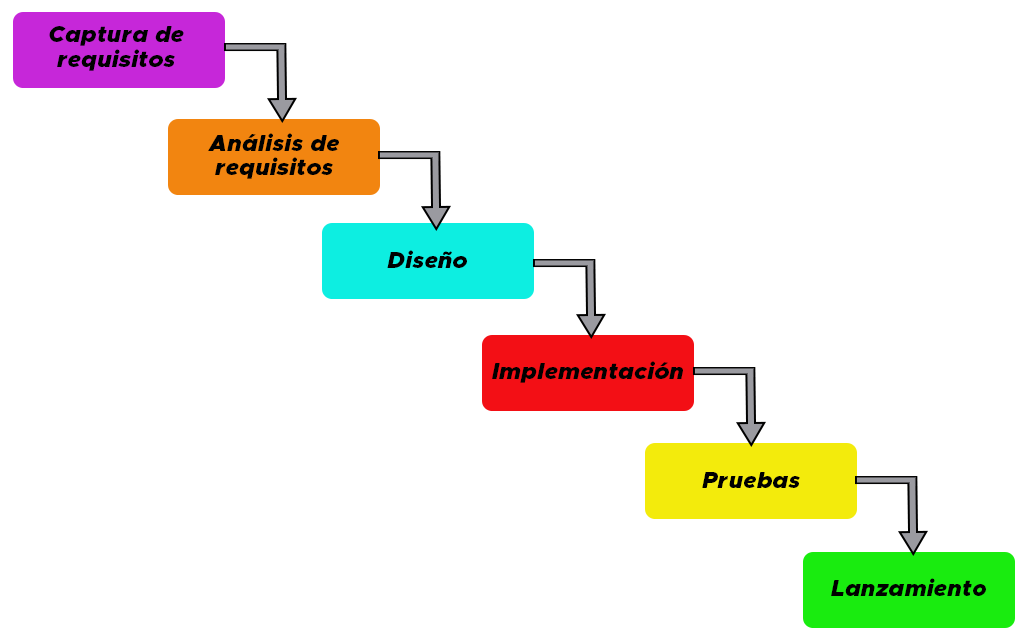
\includegraphics[width=1\textwidth]{Imagenes/Bitmap/etapasMetTradicional}\caption{Fases de una metodolog\'ia tradicional}
	%	\end{center}
	%\end{figure}
	\figura{Bitmap/etapasMetTradicional}{width=1\textwidth}{fig:etapasMetodologiaTradicional}{Fases de una metodolog\'ia tradicional}
	
	En cambio, en las metodolog\'ias \'agiles hay una lista de tareas, que se reparten entre los distintos grupos/subgrupos. \'estos suelen ser peque\~{n}os, de un tama\~{n}o m\'aximo de 10 personas. Cada tarea se trata de forma independiente, y son propensas a tener cambios (por ejemplo, es posible que una tarea inicial X, durante el desarrollo del proyecto, no se pueda realizar ya que no se ve viable), por lo que una tarea que estaba en una fase posterior s\'i puede volver a una fase previa. Todos estos cambios son los que hacen que genere valor para el cliente, por lo que la comunicaci\'on es fundamental en este tipo de metodolog\'ias.
	
	
	Hay diferentes metodolog\'ias \'agiles: \textit{XP}, \textit{Scrum}, \kanban, \textit{ScrumBan}, etc. Este proyecto seguir\'a la metodolog\'ia \kanban.


%------Segunda secci\'on: Kanban------%
\section{Kanban}
%-----------------------------------%
\label{cap3:sec:kanban}

	El t\'ermino ``\kanban``\space proviene del japon\'es, cuyo significado es ``tarjetas visuales``. Fue creado en la empresa Toyota para controlar el avance del trabajo con los materiales disponibles.
	
	Con \kanban \space puedes visualizar el trabajo hecho y por hacer, as\'i como las distintas fases por las que puede pasar una tarea, con el fin de que no se acumule el trabajo pendiente. Todo esto es posible ya que se utiliza una pizarra o tablero, ``tablero \kanban``\space (\textit{Kanban Board}). La calidad del trabajo y la productividad se ven aumentadas por la mejora del flujo de trabajo en equipo.
	
	Como uno de los objetivos de \kanban \space es saber el estado del proyecto en cada momento, y los grupos son reducidos, hay una limitaci\'on de tareas que podr\'a tener cada miembro del equipo en cada fase. Esto es el WIP (\textit{Work In Progress}).

\subsection{Tablero Kanban}
	
	Para representar las fases y las tareas se usa un tablero \kanban. Dicho tablero se divide en varias columnas que representan las distintas fases por las que puede pasar una tarea. Este tablero deber\'a tener, como m\'inimo, tres columnas:
	
	\begin{itemize}
		\item \textit{To Do}: En esta lista se tienen las tareas pendientes por realizar.
		\item \textit{Doing}: Cuando un grupo empieza a trabajar en una tarea, deber\'a moverla de ``\textit{To Do}`` a ``\textit{Doing}``.
		\item \textit{Done}: Tras saber que se ha realizado correctamente la tarea, y se ha dado por validada y aprobada, se podr\'a dar por terminada, por lo que se mover\'a a ``\textit{Done}``.
	\end{itemize}
	
	En la Figura \ref{fig:tableroKanban} se puede ver nuestro tablero \kanban \space en el inicio del proyecto. Las tres columnas que se requieren como m\'inimo est\'an presentes en nuestro tablero, pero, adem\'as, se han a\~{n}adido cuatro columnas extra:
	
	\begin{itemize}
		\item \textit{Backlog}: Corresponden con las tareas que no se pueden realizar en un presente, y que se podr\'an en un futuro.
		\item \textit{Document Review}: En esta columna se encuentran las tareas que requieren revisi\'on de memoria por parte del equipo. Estas tareas las revisar\'an quienes no hayan redactado el punto de memoria que dice la tarea.
		\item \textit{Needs Testing}: Al terminar de hacer una tarea de implementaci\'on, habr\'a que moverla de ``\textit{Doing}`` a ``\textit{Needs Testing}`` y habr\'a que pasarla en una serie de pruebas para comprobar que se ha realizado correctamente, y no da lugar a errores.
		\item \textit{Needs approval}: En esta lista se encuentran las tareas que necesitan ser aprobadas por las tutoras antes de darlas por finalizadas. Normalmente se encuentran las tareas que son de ``memoria``, aunque tambi\'en pueden aparecer de otro tipo.
	\end{itemize}
	
	\figura{Bitmap/tableroKanban}{width=1\textwidth}{fig:tableroKanban}{Tablero \kanban \space al inicio del proyecto}
	
	El WIP ser\'a de tres tareas en la columna ``\textit{In progress}``, y una en ``\textit{Needs testing}`` para cada miembro del equipo, ya que lo formamos tres personas. Hay varias excepciones en las que no se contempla el WIP, que son en ``\textit{Document Review}`` (cuando una persona realiza una tarea de redactar memoria, el resto deben revisarla en busca de incoherencias o errores en la redacci\'on, con lo cual puede haber tantas tareas de revisi\'on como de redacci\'on), y en ``\textit{Needs approval}`` (son tareas a la espera de aprobaci\'on o rechazo por parte de las tutoras).
	
	Algunas tareas podr\'an ser asignadas a varios usuarios en el caso de que sea extensa, o requiera que alguna o todas las partes necesiten hacer lo mismo. En la Figura \ref{fig:tareaVariosUsuarios}, se puede ver un ejemplo de este tipo de tarea, en el que todos los componentes del grupo han tenido que realizar un prototipo, por lo que solo se mover\'ia a ``\textit{Done}`` en el caso de que la lista est\'e completa.
	
	As\'i mismo, en la Figura \ref{fig:tableroKanban} se observa que las tareas tienen asignadas unas etiquetas de colores:
	
	\begin{itemize}
		\item \colorbox{naranja}{\textcolor{naranja}{123}} Tareas relacionadas con la memoria.
		\item \colorbox{rosa}{\textcolor{rosa}{123}} Corresponden con tareas de redacci\'on. Normalmente van en conjunto con las tareas de memoria.
		\item \colorbox{azul}{\textcolor{azul}{123}} En este color se encuentran las tareas que requieren una revisi\'on por parte del equipo. Normalmente van junto a las tareas de memoria.
		\item \colorbox{azulClaro}{\textcolor{azulClaro}{123}} Tareas que requieren un dise\~{n}o, ya sea un prototipo en papel, una interfaz de la aplicaci\'on, etc.
		\item \colorbox{rojo}{\textcolor{rojo}{123}} Tareas relacionadas con la implementaci\'on, es decir, el desarrollo de c\'odigo.
		\item \colorbox{morado}{\textcolor{morado}{123}} Aqu\'i se encuentran las tareas que requiere investigaci\'on, por parte del equipo, antes de empezar a codificar o realizar cualquier otro tipo de tarea.
		\item \colorbox{azulOscuro}{\textcolor{azulOscuro}{123}} Tareas que no corresponden con ninguna de las anteriores.
	\end{itemize}

	\figura{Bitmap/tareaVariosUsuarios}{width=1\textwidth}{fig:tareaVariosUsuarios}{Tarea asignada a varios usuarios}
	
%------\'ultima secci\'on: Tipos de pruebas------%
\section{Tipos de pruebas}
%--------------------------------------------%
\label{cap3:sec:pruebas}

	Debido a que vamos a usar componentes, es decir, ``piezas`` que son independientes entre s\'i, haremos pruebas unitarias.

\subsection{Pruebas unitarias}

	Una prueba unitaria se utiliza para comprobar que un m\'etodo implementado funciona como se esperaba. Debe cumplir una serie de caracter\'isticas:
	
	\begin{itemize}
		\item Deben ser \textbf{autom\'aticas}: se deben poder ejecutar sin que haya una intervenci\'on manual.
		\item Deben ser \textbf{completas}: es decir, deben cubrir la totalidad del c\'odigo.
		\item Deben ser \textbf{independientes}: debido a que se ha creado para comprobar una parte concreta del c\'odigo, no deber\'ia interferir con otras partes, y se deben poder ejecutar en cualquier entorno.
		\item Deben ser \textbf{repetibles}: se deben repetir todas las veces que queramos, y el resultado debe ser el mismo en todas.
	\end{itemize}

	Ventajas de las pruebas unitarias:
	
	\begin{itemize}
		\item \textbf{Aumento de la calidad} del c\'odigo: debido a que estas pruebas se ejecutan de forma regular, permite detectar errores a tiempo y poder corregirlos antes de completar el c\'odigo, y liberar la aplicaci\'on.
		\item \textbf{Facilitan los cambios}: se pueden aplicar cambios para mejorar el c\'odigo, ya que ese cambio solo afectar\'ia a una parte del c\'odigo. En el caso de que al aplicar el cambio \'este no estuviera correctamente realizado, es decir, no hiciera lo que esperase, la prueba unitaria nos avisar\'ia de que hay errores.
		\item \textbf{Reduce los tiempos} de integraci\'on: ya que podemos probar partes del c\'odigo sin disponer del c\'odigo completo.
		\item \textbf{Reduce el coste}: teniendo en cuenta que permite detectar errores tempranos, los tiempos de entrega mejoran respecto a no usarlos.
	\end{itemize}
	
	Para realizar las pruebas, hemos optado por usar \textit{Jest}\footnote{https://jestjs.io/es-ES/}, una librer\'ia de testing para \textit{Javascript}, que adem\'as es compatible con el \textit{framework} que hemos elegido (\textit{React}). \textit{Jest} tiene una instalaci\'on muy sencilla, de pocos pasos, y su configuraci\'on es m\'inima. La documentaci\'on es completa, y contiene lo necesario para poder desarrollar estos tipos de pruebas, junto con una serie de ejemplos, realizados paso a paso.
	
	Estas pruebas las desarrollar\'a y realizar\'a alguno de los miembros que no haya implementado esa parte del c\'odigo, y las har\'a cuando:
	
	\begin{enumerate}
		\item La persona que haya desarrollado el c\'odigo, haya completado dicha tarea.
		\item No tenga tareas pendientes en la columna ``\textit{Needs Testing}`` (el WIP en esa columna es de una tarea por persona).
	\end{enumerate}

	La raz\'on de esto es porque las personas que no han escrito el c\'odigo pueden sacar m\'as casos de prueba que las personas que lo han escrito.

% Variable local para emacs, para  que encuentre el fichero maestro de
% compilaci\'on y funcionen mejor algunas teclas r\'apidas de AucTeX
%%%
%%% Local Variables:
%%% mode: latex
%%% TeX-master: "../Tesis.tex"
%%% End: